Following the submission of the verilog designs on September 5th, 2023, the Tiny Tapeout team began the process of verification. 
The verification process consisted of a series of proprietary tests to ensure that the designs were correct and that they would be able to be fabricated.
Subsequently, the Tiny Tapeout team reached out to confirm the approval for fabrication. The expected delivery date for the fabricated chips is on February 15th, 2024.

The use of Github has allowed the design submission process to become more automated and streamlined. The use of Github has also allowed the Tiny Tapeout team to develop 
interesting and innovative tools to aid in the intricacies of the designs making process. One of these tools is a 2D viewer that allows the user to view the final 
layout of the design on the die and a 3D viewer that allows the user to see the different layers of the design to further understand the complexity of what is behind the 
fabrication of a chip. The 2D and 3D views of each of the design submitted are shown in the figures \ref*{fig:delay_Layout}, \ref*{fig:ASCII_Layout}, \ref*{fig:Pong_Layout} and \ref*{fig:PWM} 
were generated on the git repository of the respective git projects for each of the designs.

\begin{figure}[H]
    \centering
    \begin{subfigure}[b]{0.45\textwidth}
        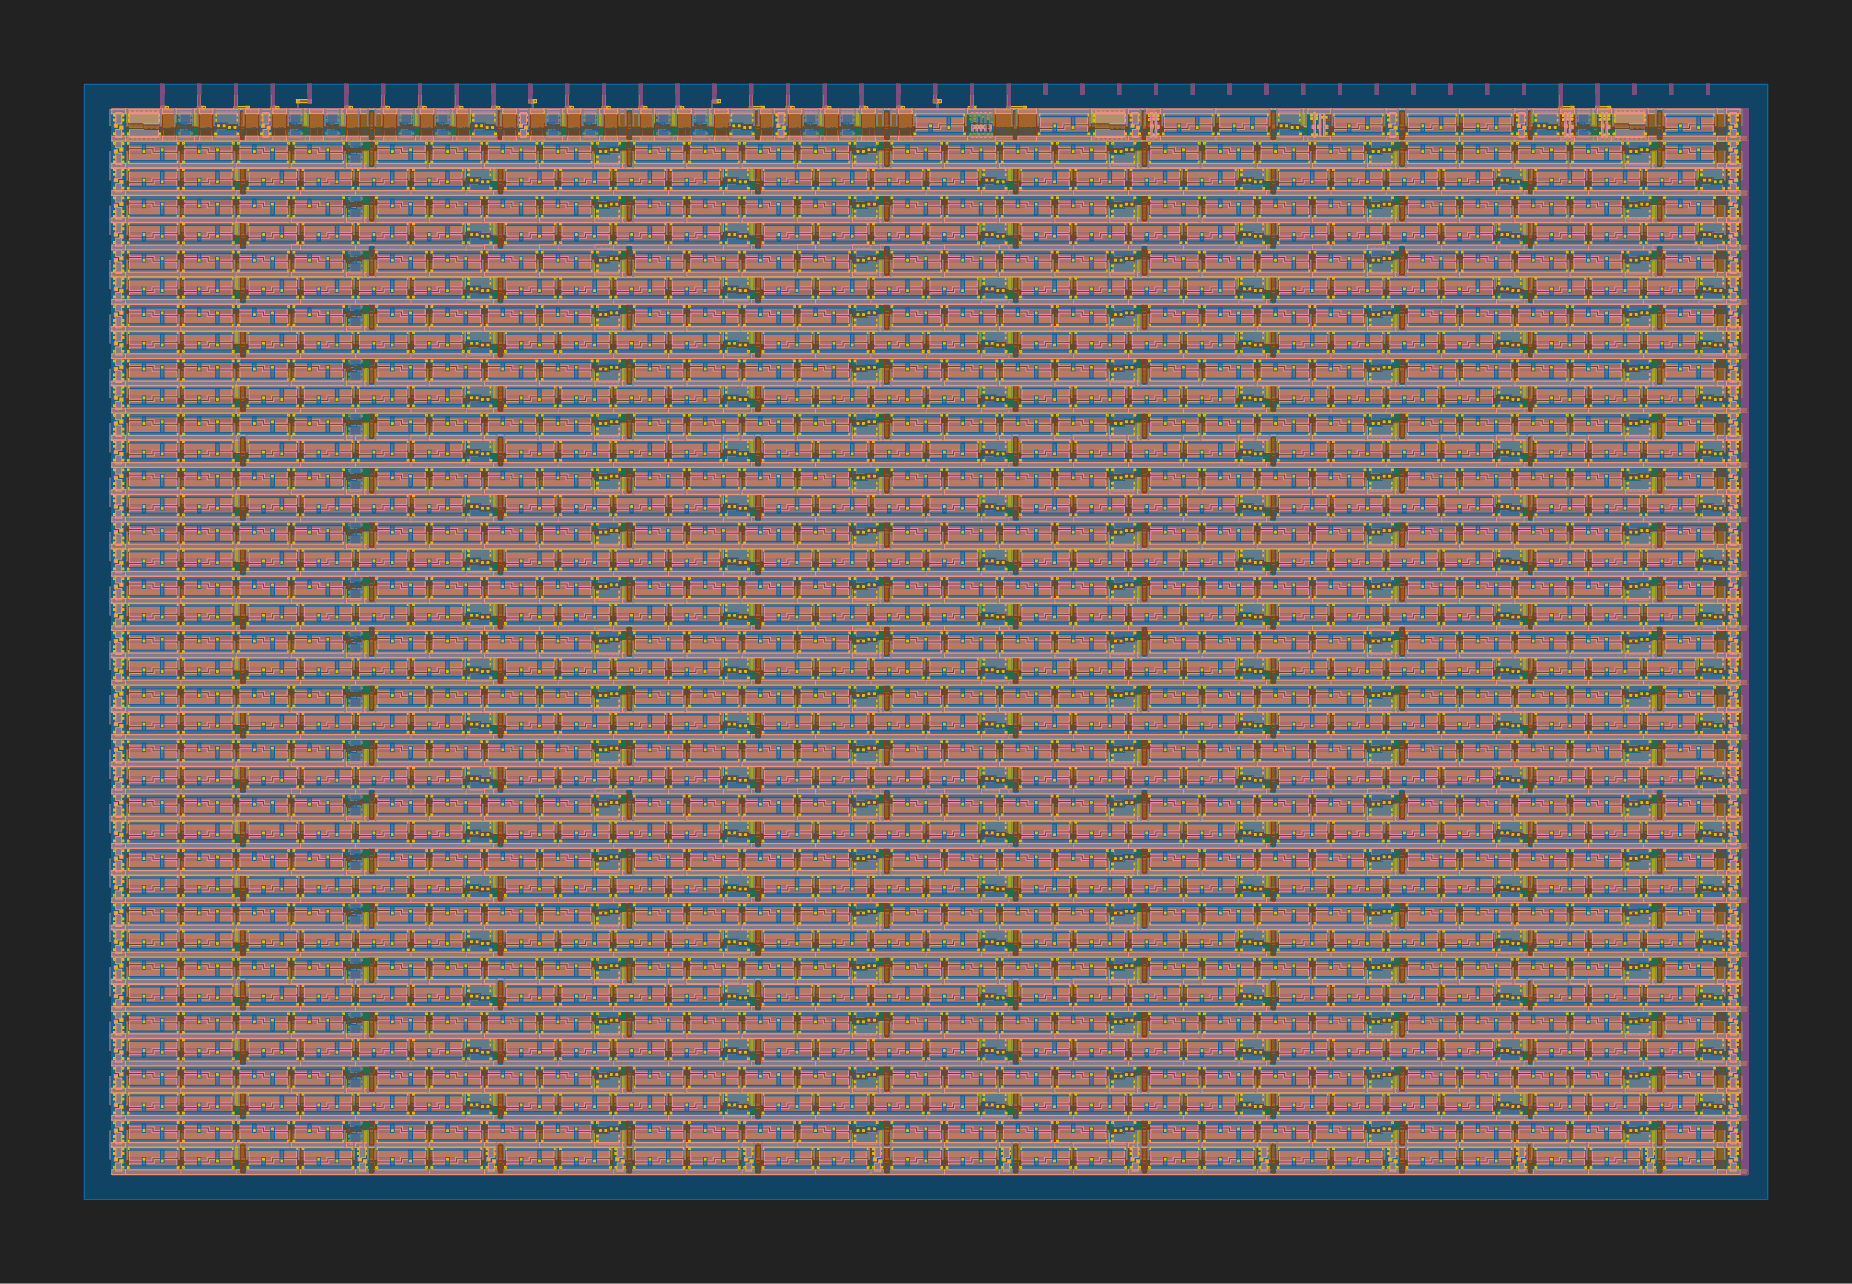
\includegraphics[width=\linewidth]{Pictures/Result_Delay_2D_View.png}
        \caption{View 2D}\label{fig:delay_2D}
    \end{subfigure}
    \begin{subfigure}[b]{0.45\textwidth}
        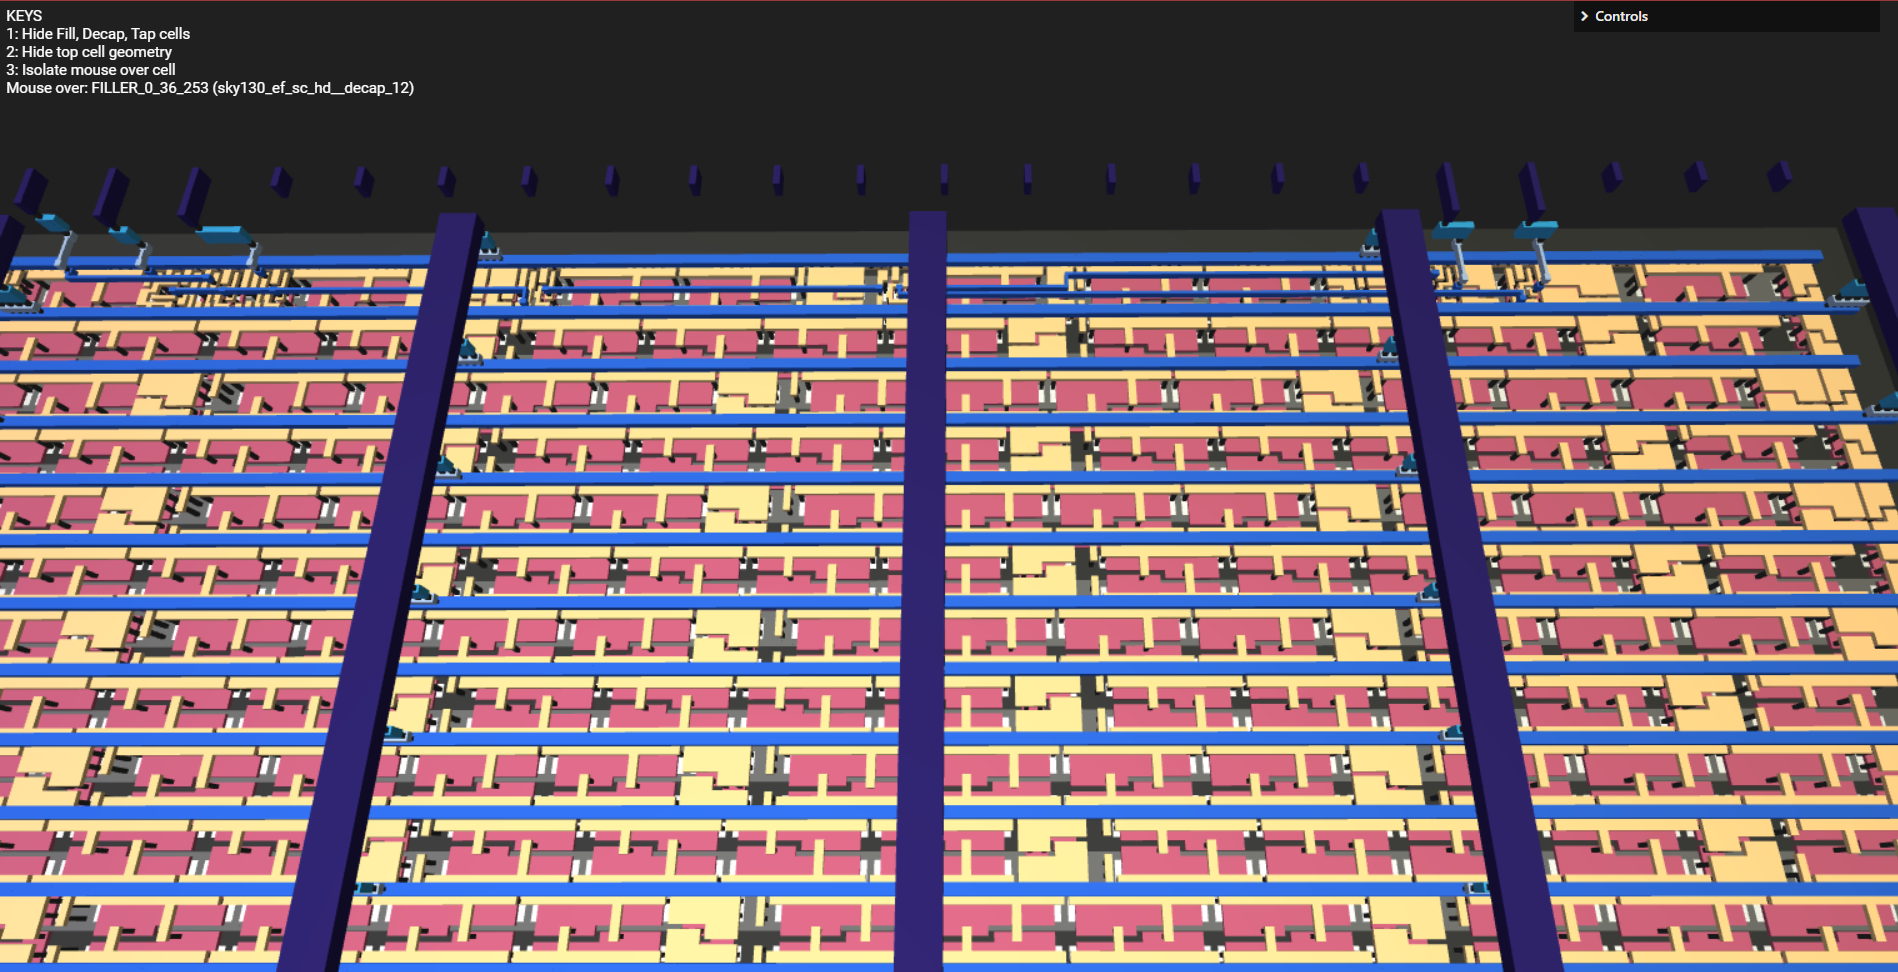
\includegraphics[width=\linewidth]{Pictures/Result_Delay_3D_View.png}
        \caption{View 3D}\label{fig:delay_3D}
    \end{subfigure}
    \caption{multistage path for delay measurements layout}\label{fig:delay_Layout}
\end{figure}

\begin{figure}[H]
    \centering
    \begin{subfigure}[b]{0.45\textwidth}
        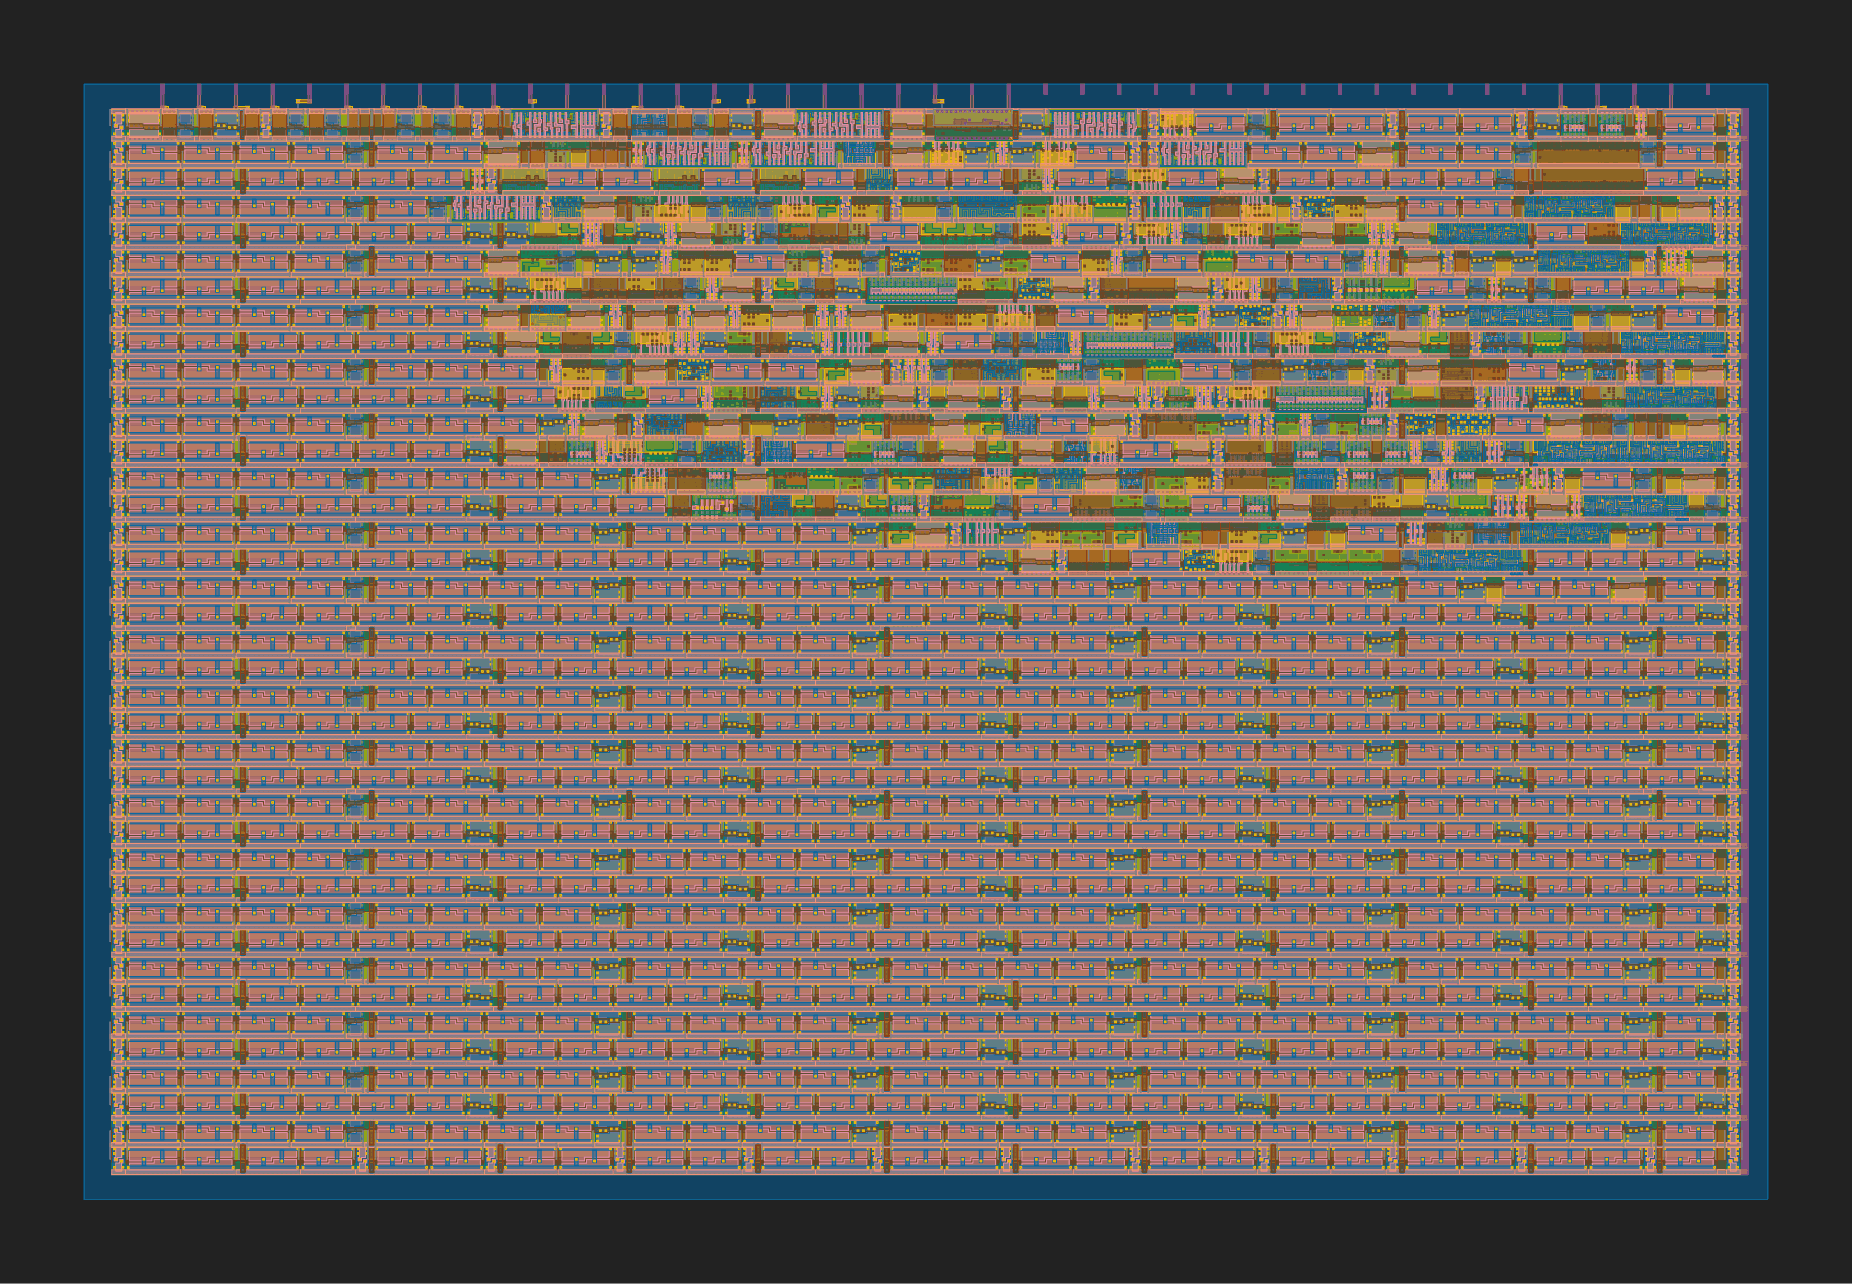
\includegraphics[width=\linewidth]{Pictures/Result_ASCII_2D_View.png}
        \caption{View 2D}\label{fig:ASCII_2D}
    \end{subfigure}
    \begin{subfigure}[b]{0.45\textwidth}
        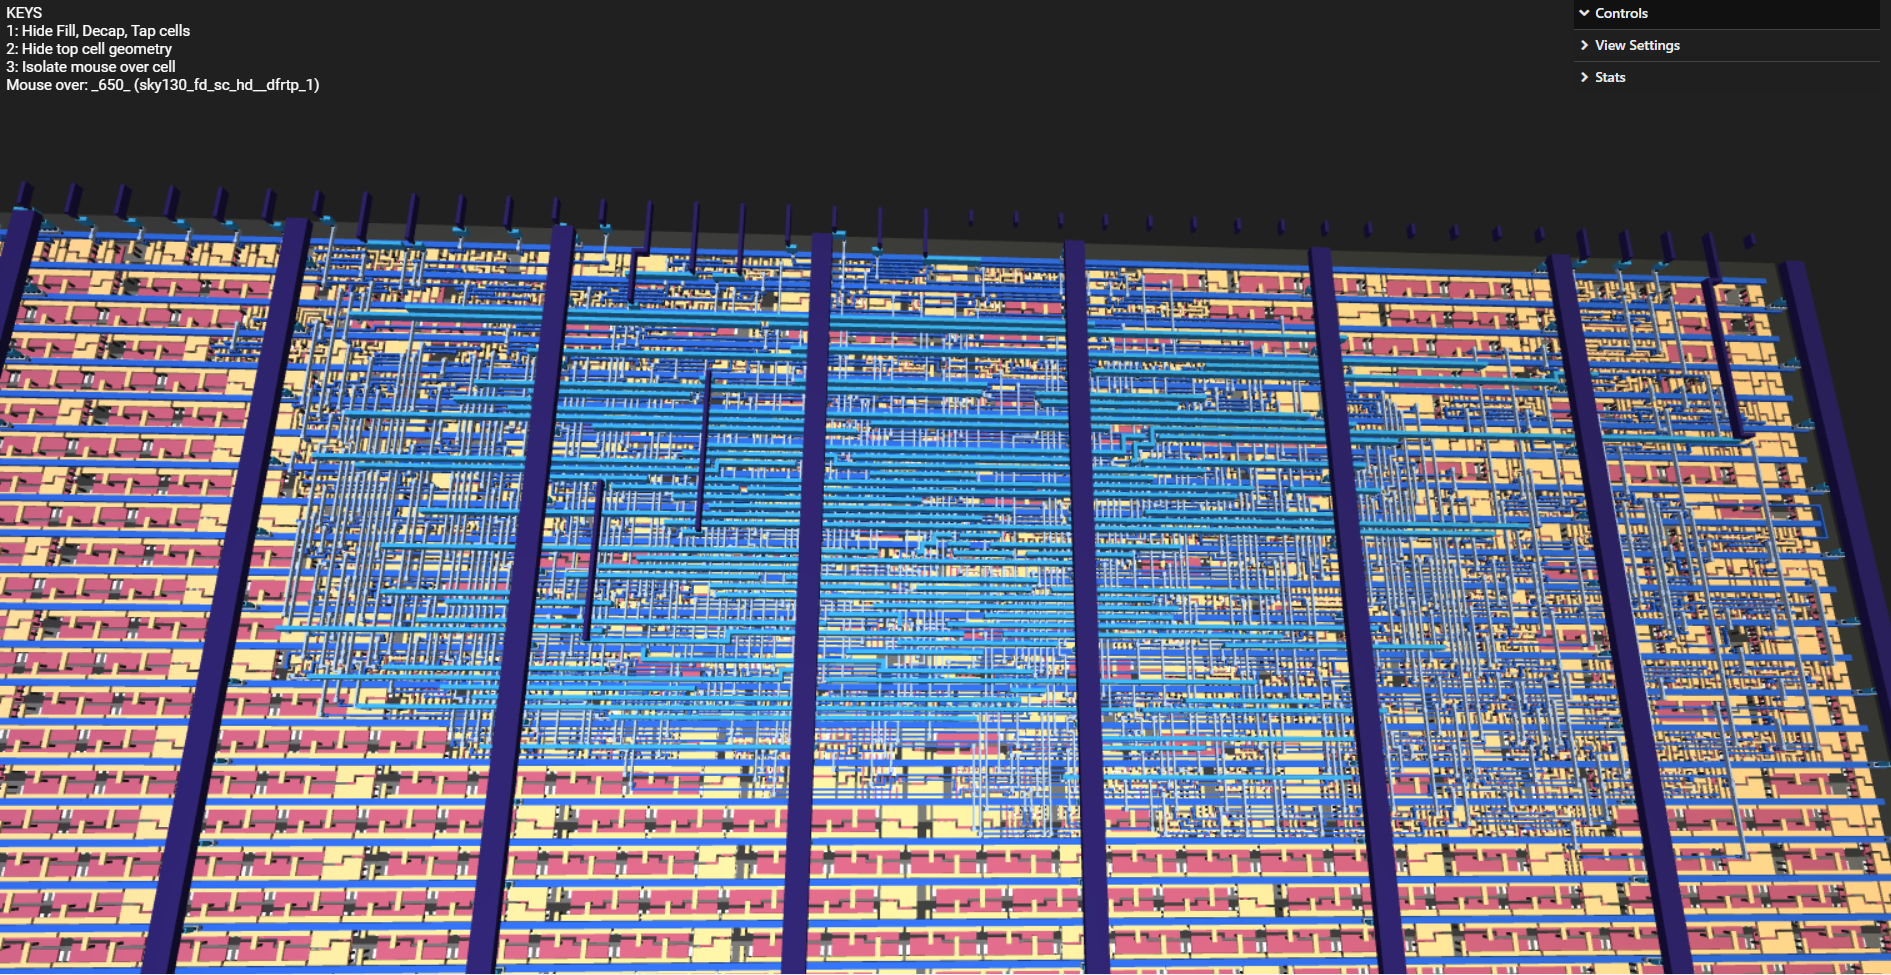
\includegraphics[width=\linewidth]{Pictures/Result_ASCII_3D_View.png}
        \caption{View 3D}\label{fig:ASCII_3D}
    \end{subfigure}
    \caption{ASCII text printer circuit layout}\label{fig:ASCII_Layout}
\end{figure}

\begin{figure}[H]
    \centering
    \begin{subfigure}[b]{0.45\textwidth}
        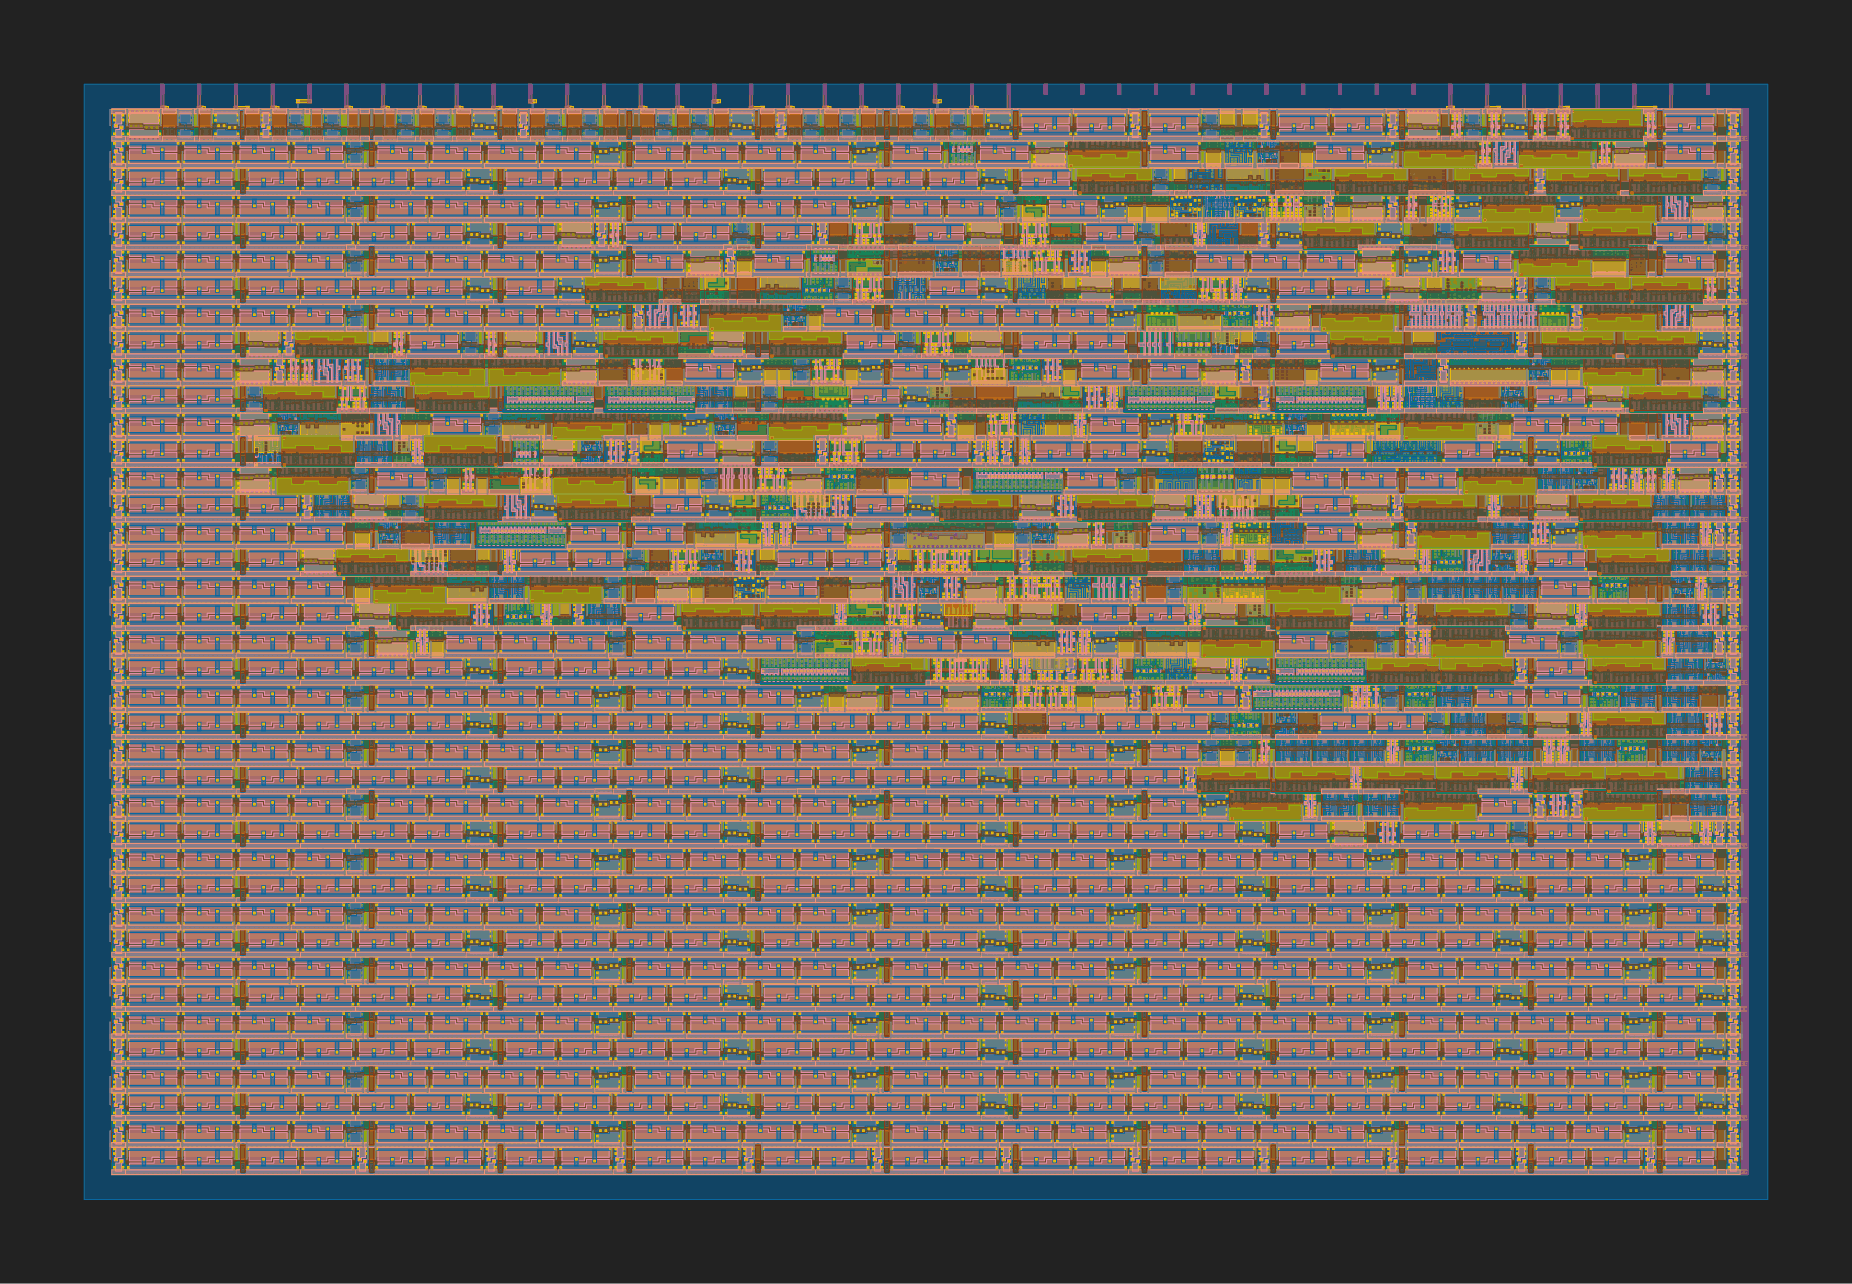
\includegraphics[width=\linewidth]{Pictures/Result_Pong_2D_View.png}
        \caption{View 2D}\label{fig:pong_2D}
    \end{subfigure}
    \begin{subfigure}[b]{0.45\textwidth}
        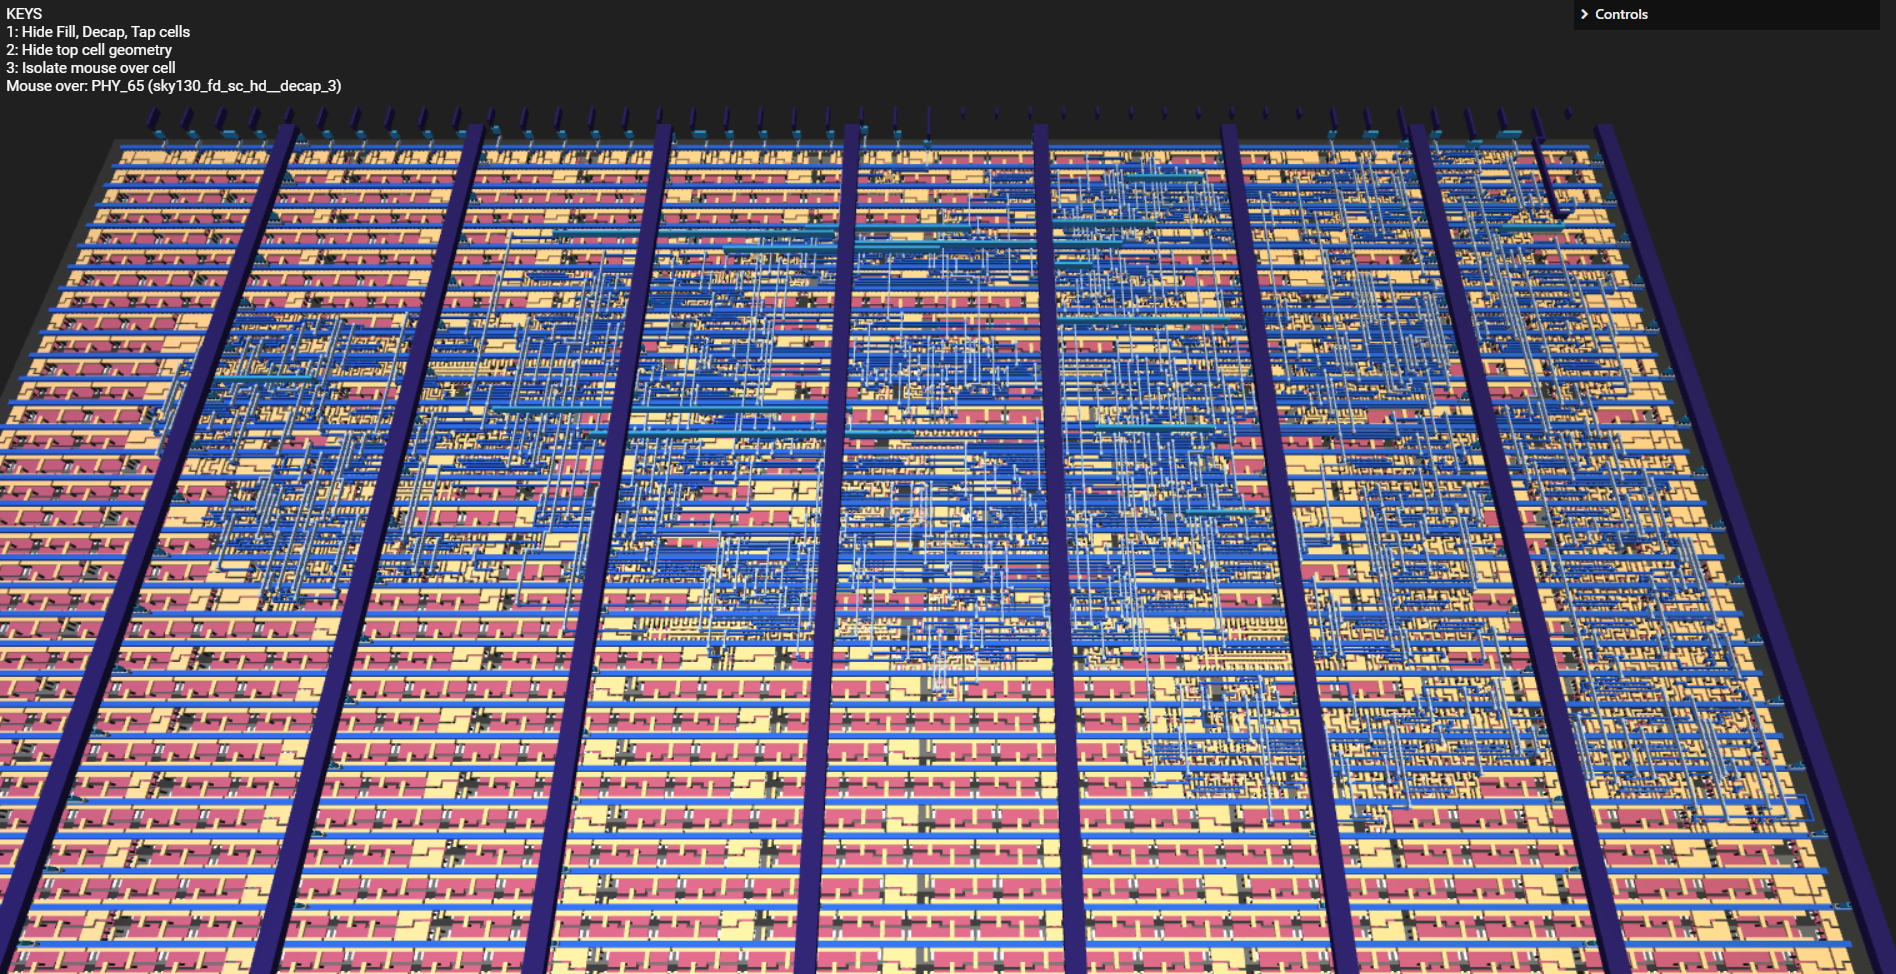
\includegraphics[width=\linewidth]{Pictures/Result_Pong_3D_View.png}
        \caption{View 3D}\label{fig:pong_3D}
    \end{subfigure}
    \caption{The Pong game layout}\label{fig:Pong_Layout}
\end{figure}

\begin{figure}[H]
    \centering
    \begin{subfigure}[b]{0.45\textwidth}
        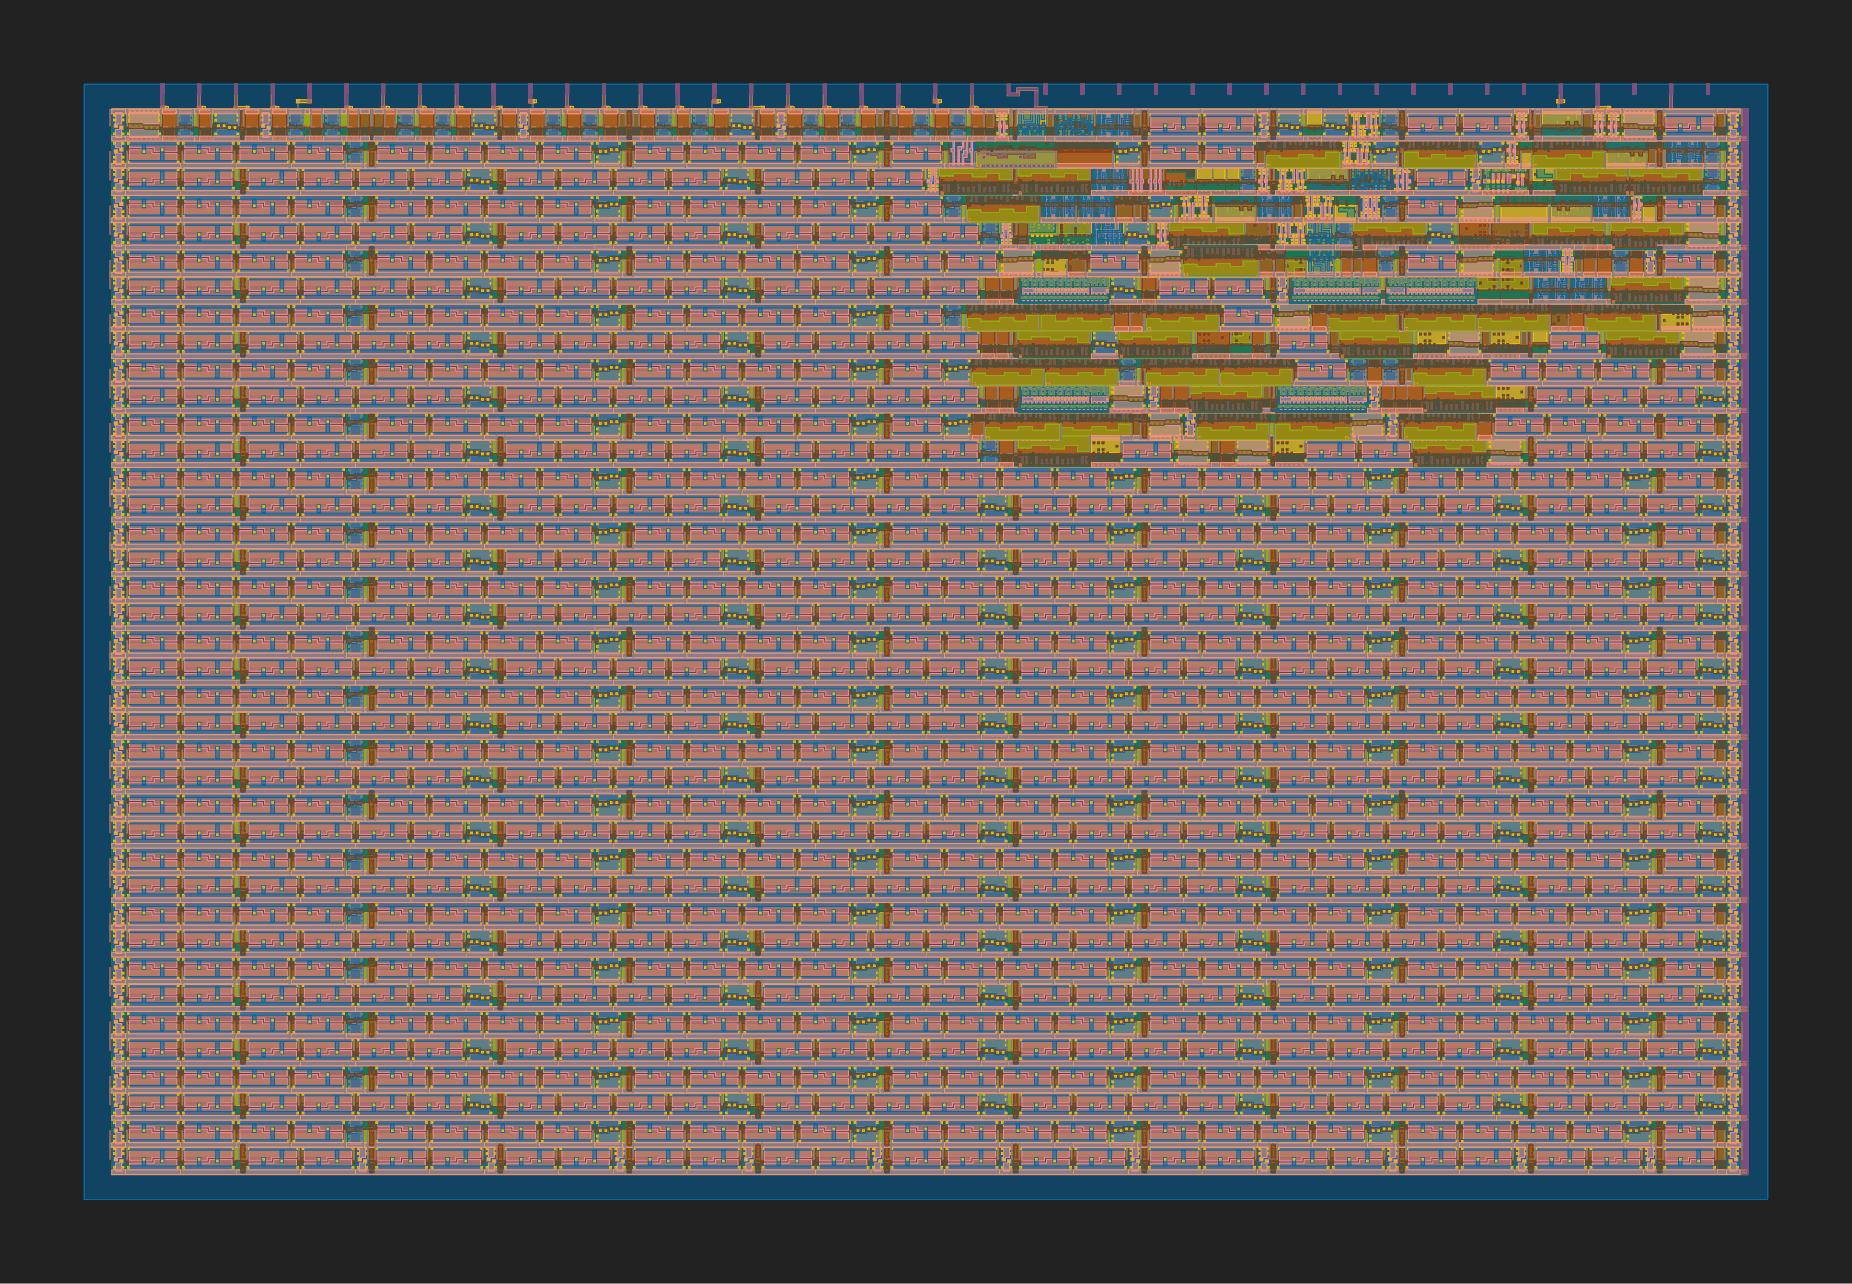
\includegraphics[width=\linewidth]{Pictures/Result_PWM_2D_View.png}
        \caption{View 2D}\label{fig:PWM_2D}
    \end{subfigure}
    \begin{subfigure}[b]{0.45\textwidth}
        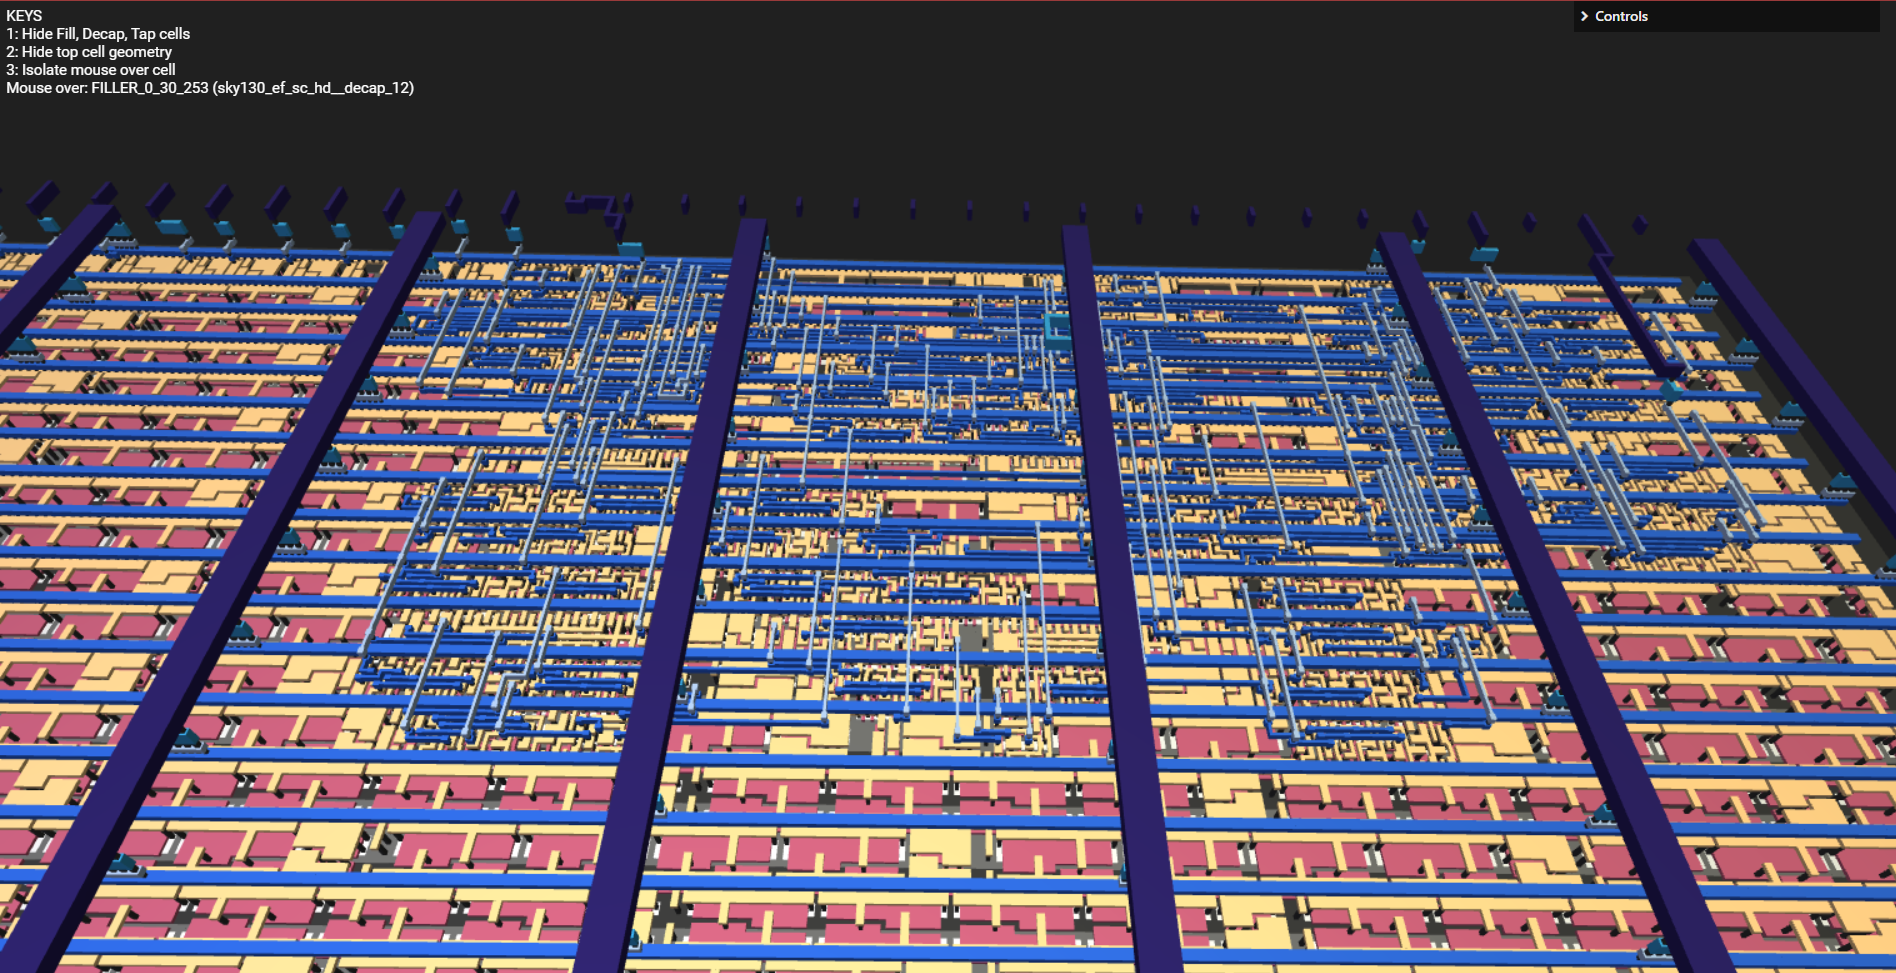
\includegraphics[width=\linewidth]{Pictures/Result_PWM_3D_View.png}
        \caption{View 3D}\label{fig:PWM_3D}
    \end{subfigure}
    \caption{Pulse Width Modulation generator layout}\label{fig:PWM}
\end{figure}

% Please add the following required packages to your document preamble:
% \usepackage{graphicx}


For a more in deep illustration on the complexity of the designs, figure \ref*{fig:Specific_Layout} 
has been included to showcase the different layers of the Pulse Width Modulation generator design.
The grey rectangles that can be observed in the figure are the N-wells for the transistors, 
the diffusion junction are the white rectangles, the pink rectangles are the polysilicon layers, 
the blue rectangles are the interconnect. 


\begin{figure}[H]
    \centering
        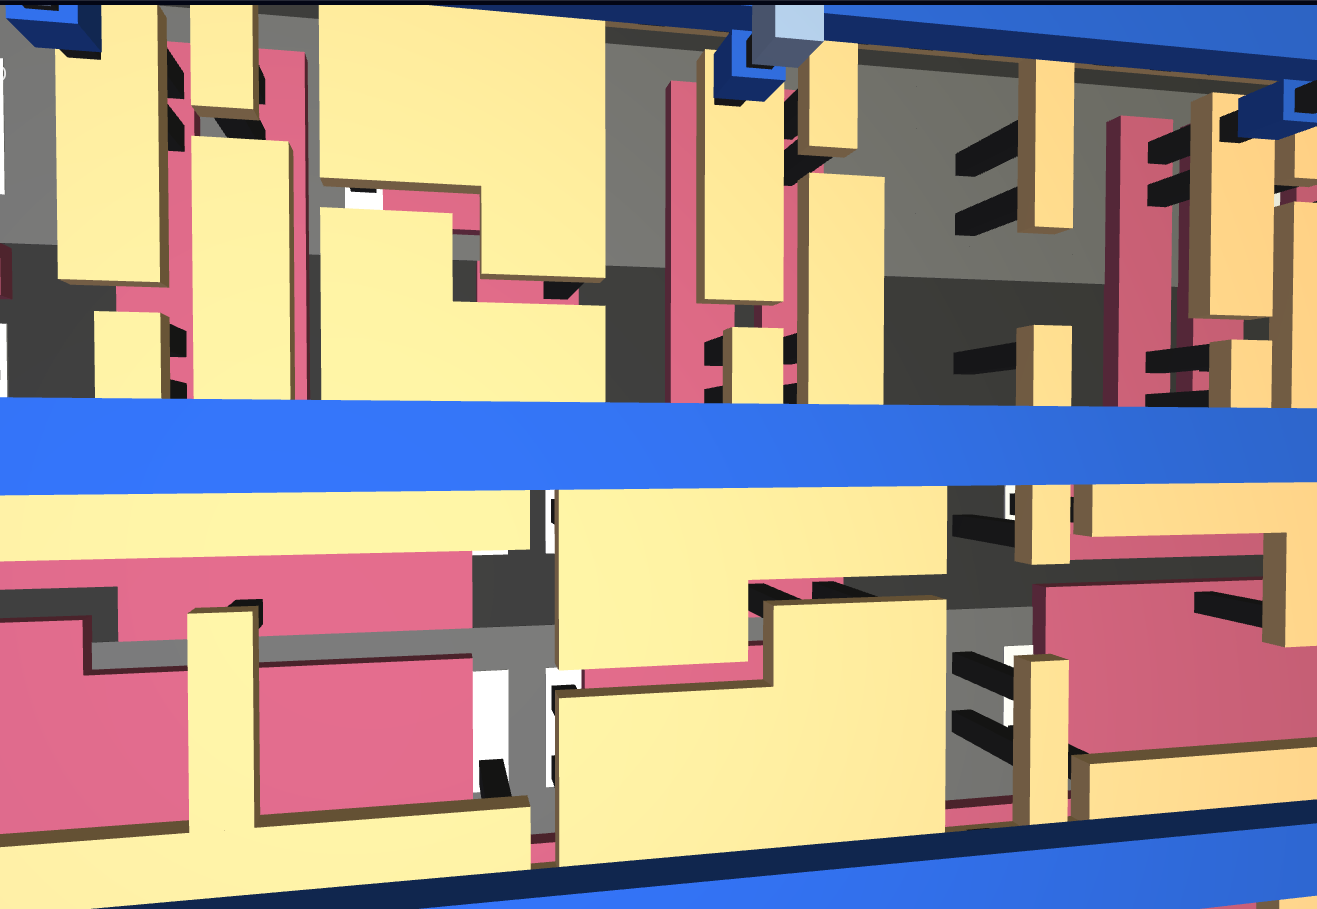
\includegraphics[width=\linewidth]{Pictures/Specific_Layout.png}
    \caption{Pulse Width Modulation generator layout}\label{fig:Specific_Layout}
\end{figure}

The Tiny Tapeout initiative has some limitations that are given by the nature of the project, one of 
the most important limitations to take inconsideration is the size of the die that each of the participants has 
to work with, due to this initiative being a multi-project wafer the size of the die is limited to 160um x 100um. 
This sizes may vary depending on the year of the initiative, due to how many projects are being submitted for fabrication. 
Table \ref*{tab:PorcentUtil} shows the percentage of the die that was utilized by each of the designs submitted.

\begin{table}[H]
    \centering
    \resizebox{\columnwidth}{!}{%
    \begin{tabular}{cc}
    \hline
    Circuit                                 & Porcentage utilize(\%) \\ \hline
    Multy stage path for delay measurements & 0.63                  \\
    ASCII Text Printer Circuit              & 17.87                 \\
    Implementation of the Pong game         & 28.82                 \\
    Pulse Width Modulation Generator        & 9.59                  \\ \hline
    \end{tabular}%
    }
    \caption{Porcentaje utilize in length of waver per circuit}\label{tab:PorcentUtil}
    \end{table}

    